\appendix
\renewcommand{\thetable}{S\arabic{table}}
\renewcommand{\thefigure}{S\arabic{figure}}
\setcounter{table}{0}\setcounter{figure}{0}
\section*{Supplementary material}
\addcontentsline{toc}{section}{Supplementary material}

The analyses below started the project. They concern specific estimators, simulators and regimes, and their conclusions are stated at that level. All simulation results use the seeds listed. ``Diagnostic re-implementations'' of published method families (PHOENIX-, DCDI-, CellOracle- and GENIE3-style) implement only each method's core idea in our code. They are controls, not evaluations of the original software.

\paragraph{Metric definitions (all simulations).} The candidate-edge universe is every ordered pair $(j\to i)$ of distinct \emph{measured} genes: $70\times69=4{,}830$ pairs in the 80-gene simulator, of which about 114 are true edges. AUROC and average precision (AUPRC) are computed over this universe. AUPRC$\times$ is AUPRC divided by the base rate (true edges / candidates), so 1 = random. $E$ is the number of true edges among measured genes; ``top-$E$'' metrics use the $E$ highest-scored pairs. ``Indirect'' pairs have a directed path of length $\ge2$ (through any gene, measured or hidden) and no direct edge.

\subsection*{S1. Thermodynamic occupancy model}
\textbf{Occupancy calibration.} For each TF, $E_\text{thr}$ is the 10$^{-4}$ quantile of PWM energies on 400{,}000 background positions with promoter base composition (a FIMO-like threshold). Occupancy uses $\mu=E_\text{thr}+\{-4,-2,0\}$ ($-2$ pre-registered as default). ProBound models (MotifCentral v1.0.0; human model preferred, lowest fit id) were rescaled to a maximum log-affinity of 0.

\textbf{T1, synthetic genome} (1{,}500 genes, 20 JASPAR TFs, 3 seeds). Two different comparisons are reported.
\begin{itemize}
\item Over all targets, summed occupancy at $\mu=E_\text{thr}$ reached AUROC 0.959 vs 0.820 for the maximum motif score.
\item Restricted to weak-cluster targets vs non-targets, occupancy reached 0.968 vs 0.647.
\end{itemize}
A fitted occupancy model recovered TF activities $\mu$ (Spearman 0.976).

\textbf{T3, cell-state $\mu$ (K562 vs HepG2).} Test $R^2$ for log expression: 0.172 (accessibility only), 0.185 (fixed $\mu$), 0.188 (state-specific $\mu$). For the HepG2$-$K562 \emph{difference}, $R^2$ rose from 0.006 (fixed $\mu$) to 0.017 (state-specific $\mu$), an improvement of 0.011.
The inferred $\Delta\mu$ did not correlate with independent proxies (Spearman 0.06--0.09, permutation $p>0.29$).

\textbf{ProBound vs JASPAR} (122 TFs). Binding AUROC was higher with ProBound for 69--73\% of TFs (paired Wilcoxon $p<10^{-7}$), by about 0.02. There was no gain for function (13 TFs).

\subsection*{S2. Latent neural ODE on a three-gene cascade, and a 10-gene toy}
\textbf{Simulation.} A$\to$B$\to$C with Hill kinetics ($K=0.6$, $n=2$), Euler--Maruyama ($dt=0.005$). 200 cells (150 train), 41 observations at interval 0.2, measurement noise 5\% or 20\% of the per-gene s.d.
\textbf{Model.} Gene-aligned latent states (residual per-gene MLP encoder and decoder) and dynamics $dz/dt=W\sigma(a(z-c))-\operatorname{softplus}(g)z+b$ with $\operatorname{diag}(W)=0$. Free latent units are initialised from a learned constant (``from start'') or from $(x_t,x_t-x_{t-1})$.
Loss: $K$-step rollout MSE (4 Euler substeps per interval) + reconstruction + $\lambda\|W\|_1$. Adam, learning rate $10^{-2}$, cosine schedule, 2{,}000 iterations (1{,}200 for from-start runs). $\lambda$ grid $\{0,10^{-5},\dots,10^{-2}\}$; 3 seeds. An edge is called if its strength (|$W_{ij}$| $\times$ range of $j$'s activation along the rollout) is $\ge10\%$ of the largest.
\textbf{Results.} With all genes observed, the exact graph was recovered in 57--71\% of settings. With B hidden, the shortcut A$\to$C was called in 81--100\% of fits. With knockdowns of the hidden B supplied and modelled (applied to a latent unit with a learned efficiency), A$\to h\to$C was recovered without the shortcut in 75\% of settings (latent--B correlation 0.975). With the same knockdowns unmodelled, the shortcut was always called.
In a 10-gene toy, a binding prior raised AUROC from 0.749 to 0.947 (0.962 with knockdown-aware fitting). Two indirect edges stayed in the top 9 until the intermediate TF was itself knocked down.

\subsection*{S3. 80-gene simulator: ablations and experiment selection}
\textbf{Simulator} (in-house, SERGIO-style): 80 genes (16 TFs, 8 non-TF regulators, 56 targets; about 140 edges; TF cascades of depth $\ge3$; 70\% activators). Per-edge Hill coefficient $n\in\{1..4\}$ and threshold $K\sim U(0.5,2)$; decay $U(0.5,1)$; process noise 0.05; a hidden cell-size factor; Poisson counts with log-normal library size; noisy labelling velocity (1$\times$ s.d.); 10 unmeasured genes; 1{,}500 wild-type cells and 80 cells per knockdown, with efficiency $U(0.05,0.3)$. Seeds 0--9.
\textbf{BOND-V:} nodewise adaptive lasso \citep{zou2006} (BIC) of velocity on Hill features $\phi(x_j)=x_j^2/(K_j^2+x_j^2)$, $K_j=\operatorname{median}(x_j)$, plus a decay term. Features are standardised before division by the penalty factor $1-\alpha p_{ij}$. Each gene's own-knockdown cells are dropped from its equation.
Ablation results (AUPRC$\times$, 10 seeds):
\begin{itemize}
\item full model 18.6; without prior 15.5; ignoring interventions 17.6; static (no velocity) 16.4;
\item knockdown mean-difference 26.4, but with 36\% indirect edges in its top $E$;
\item diagnostic re-implementations: CellOracle-style 8.9, GENIE3-style \citep{huynh2010genie3} 5.7.
\end{itemize}
Disambiguation-driven knockdown selection beat random and hub-based choice in 10/10 seeds (area under the AUPRC$\times$ coverage curve $+0.95\pm0.67$ vs random). It was not tested on real data.

\begin{figure}[h]
\centering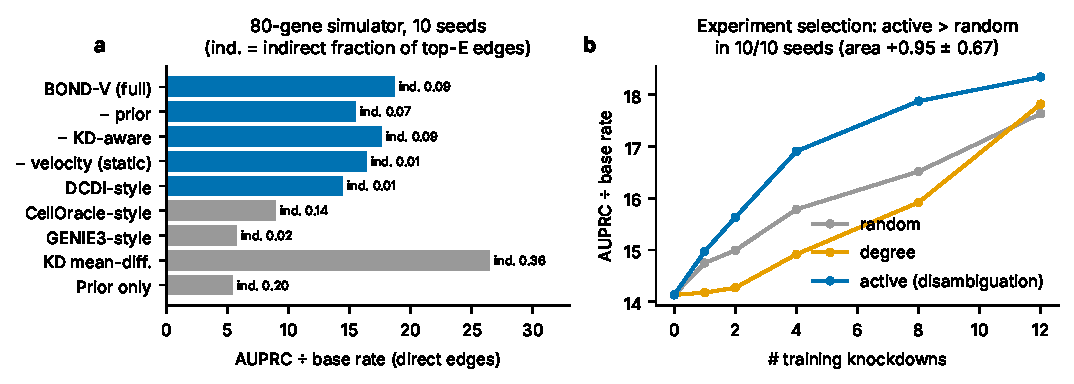
\includegraphics[width=0.9\textwidth]{figures/fig2_medium_synthetic.pdf}
\caption{\textbf{80-gene simulator.} (a) Ablations and diagnostic re-implementations. (b) Knockdown selection strategies.}
\end{figure}

\subsection*{S4. Linear SEM on real held-out knockdowns}
On 203 strongly knocked-down Replogle genes, a knockdown-aware steady-state linear SEM predicted held-out knockdown profiles with correlation $0.012\pm0.298$, against $0.422\pm0.402$ for the mean training profile. ChIP and motif priors did not change this.

\subsection*{S5. A lag-feature ridge detector of hidden regulators (memory)}
\textbf{Scope.} This tests one estimator: ridge regression of an observed gene's 5-step-ahead change on the current observed state, with and without lags of 1, 2, 4 and 8 samples. It is not a test of memory-function methods in general \citep{herrera2018memory,zhang2019memory,biswas2021memory}.
\textbf{Simulation.} Measurement-noise levels are relative to each gene's simulated within-trajectory fluctuation s.d. They are not calibrated against any real assay, so we do not call any level ``realistic''.
\textbf{Results.} With regulator process noise four times that of other genes and clean data, the detector ranked children of hidden regulators above other genes (AUROC 0.84 vs 0.51 with nothing hidden; Table~\ref{tab:s_f3}). It failed with weaker regulator fluctuations, with measurement noise $\ge0.5\times$ the fluctuation s.d., and with sampling intervals $\ge0.25$. Estimates of the hidden regulator's timescale and of the number of hidden regulators (lagged-residual rank) failed.

\begin{table}[h]
\centering\small
\caption{\textbf{Lag-feature ridge detector} (AUROC; 80-gene time courses; seeds 0--9 or 0--5).}
\label{tab:s_f3}
\begin{tabular}{lcc}
\toprule
Detector / condition & AUROC (mean $\pm$ sd over seeds) & seeds \\
\midrule
Memory gain, 2 hidden regulators (clean) & 0.836 $\pm$ 0.169 & 10 \\
Same genes, nothing hidden (control) & 0.512 $\pm$ 0.114 & 10 \\
Snapshot detector ($1-R^2$), hidden regulators & 0.374 $\pm$ 0.068 & 10 \\
Memory gain, weak regulator fluctuations & 0.543 $\pm$ 0.127 & 10 \\
Memory gain, measurement noise 0.1$\times$ fluct.\ sd & 0.875 $\pm$ 0.129 & 6 \\
Memory gain, measurement noise 0.25$\times$ fluct.\ sd & 0.705 $\pm$ 0.151 & 6 \\
Memory gain, measurement noise 0.5$\times$ fluct.\ sd & 0.487 $\pm$ 0.052 & 6 \\
Memory gain, measurement noise 1.0$\times$ fluct.\ sd & 0.444 $\pm$ 0.058 & 6 \\
\quad control (nothing hidden), noise 0.25 & 0.545 $\pm$ 0.103 & 6 \\
\quad control (nothing hidden), noise 0.5 & 0.535 $\pm$ 0.050 & 6 \\
Noise 0.5 + causal smoothing (attempted fix) & 0.531 $\pm$ 0.105 & 6 \\
Sampling interval 0.05 (clean) & 0.807 $\pm$ 0.072 & 4 \\
Sampling interval 0.1 (clean) & 0.881 $\pm$ 0.072 & 4 \\
Sampling interval 0.25 (clean) & 0.664 $\pm$ 0.138 & 4 \\
Sampling interval 0.5 (clean) & 0.463 $\pm$ 0.253 & 4 \\
Sampling interval 1.0 (clean) & 0.436 $\pm$ 0.024 & 4 \\
Sampling interval 2.0 (clean) & 0.433 $\pm$ 0.037 & 4 \\
\bottomrule
\end{tabular}\\[2pt]
\begin{minipage}{0.9\textwidth}\footnotesizeMedian memory gain (fraction of held-out error removed by the past), clean main condition: genes with a hidden regulator 0.027 $\pm$ 0.023, other genes -0.007 $\pm$ 0.002. Oracle gain from adding the true hidden state: 0.093 $\pm$ 0.054 vs -0.001 $\pm$ 0.000.\end{minipage}
\end{table}
\begin{figure}[h]
\centering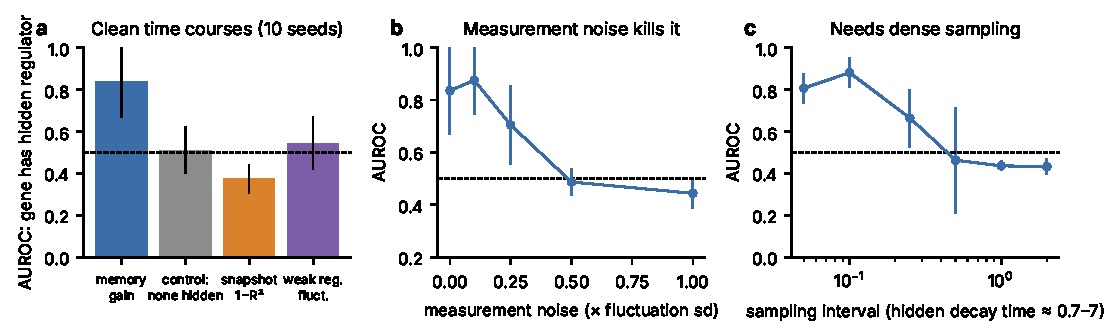
\includegraphics[width=\textwidth]{figures/fig5_memory.pdf}
\caption{\textbf{Lag-feature ridge detector.} (a) Clean, dense time courses. (b) Measurement noise relative to simulated fluctuations. (c) Sampling interval.}
\end{figure}

\subsection*{S6. Intervention-induced indirect edges (errors-in-variables)}
For A$\to$B$\to$C with $B=bA+\varepsilon_B$, $C=cB+\varepsilon_C$ and B measured as $\tilde B=B+e$, regressing C on $(A,\tilde B)$ gives $\beta_{A\to C}=cb\lambda$, $\lambda=\sigma_e^2/(\sigma_e^2+\operatorname{Var}(B|A))$ \citep{fuller1987}.
Perturbing A leaves $\beta$ unchanged but makes it easier to detect. Perturbing B lowers $\lambda$ (Table~\ref{tab:s_f4three}).
In the 80-gene simulator, perturbing the source raised the indirect-call rate only slightly, and hidden mediators dominated (Table~\ref{tab:s_f4net}). A simple identifiability flag was modestly informative (Table~\ref{tab:s_f4flag}).

\begin{table}[h]\centering\small
\caption{\textbf{Three-gene check} ($b=c=1$, $\sigma_B=\sigma_C=\sigma_e=0.5$, $n=2{,}000$, 300 replicates).}\label{tab:s_f4three}
\begin{tabular}{lcccc}
\toprule
Condition & theory $cb\lambda$ & simulated coefficient & mean $t$ & Lasso selects A$\to$C \\
\midrule
observational & 0.500 & 0.497 $\pm$ 0.024 & 21.0 & 1.00 \\
perturb A & 0.500 & 0.500 $\pm$ 0.022 & 23.9 & 1.00 \\
perturb B & 0.100 & 0.099 $\pm$ 0.017 & 5.5 & 1.00 \\
perturb A and B & 0.100 & 0.076 $\pm$ 0.011 & 6.8 & 1.00 \\
\bottomrule
\end{tabular}\end{table}
\begin{table}[h]\centering\small
\caption{\textbf{Indirect pairs called as edges} by perturbation status (BOND-V without prior; seeds 0--9 $\times$ 3 random halves of the perturbation set).}\label{tab:s_f4net}
\begin{tabular}{llcc}
\toprule
Source (regulator) & 2-hop mediator & indirect pairs & \% called (top-$E$), $\pm$ seed sd \\
\midrule
source perturbed & mediator unperturbed & 874 & 5.9 $\pm$ 3.2 \\
source perturbed & mediator perturbed & 881 & 4.9 $\pm$ 3.4 \\
source perturbed & mediator hidden & 175 & 14.9 $\pm$ 14.3 \\
source perturbed & longer path only & 1709 & 0.2 $\pm$ 0.3 \\
source unperturbed & mediator unperturbed & 779 & 5.1 $\pm$ 1.9 \\
source unperturbed & mediator perturbed & 862 & 4.3 $\pm$ 3.3 \\
source unperturbed & mediator hidden & 179 & 17.3 $\pm$ 12.5 \\
source unperturbed & longer path only & 1723 & 0.3 $\pm$ 0.5 \\
\bottomrule
\end{tabular}\end{table}
\begin{table}[h]\centering\small
\caption{\textbf{Identifiability flag} (edge $j\to i$ flagged if some unperturbed $m$ has predicted $j\to m$ and $m\to i$ edges among the top $2E$).}\label{tab:s_f4flag}
\begin{tabular}{lc}
\toprule
Quantity & Value \\
\midrule
n predicted edges & 3426 \\
fraction flagged & 0.437 \\
precision flagged & 0.273 \\
precision unflagged & 0.441 \\
indirect frac flagged & 0.089 \\
indirect frac unflagged & 0.054 \\
share of indirect FPs that are flagged & 0.561 \\
share of TPs flagged & 0.324 \\
precision source perturbed & 0.835 \\
precision source unperturbed & 0.208 \\
precision regulator source perturbed & 0.835 \\
precision regulator source unperturbed & 0.717 \\
n edges from unperturbed regulators & 739 \\
n edges from perturbed & 873 \\
fraction of edges from non regulators & 0.529 \\
precision flagged among regulator sources & 0.711 \\
precision unflagged among regulator sources & 0.820 \\
\bottomrule
\end{tabular}\end{table}

\subsection*{S7. Prior forms and imperfect regulator masks}
With an \emph{exact} regulator list, a hard identity mask raised AUPRC$\times$ from 15.5 (no prior) to 22.2, and adding a soft site-level binding prior on top gave 23.2 (Table~\ref{tab:s_f5}). The reading is ``mask first; a site prior adds a little on top''.
A hard binding-site mask capped recall at 25\% and was harmful.
With imperfect masks (Table~\ref{tab:s_masks}, Fig.~\ref{fig:s_masks}), each missing regulator cost far more than each false one, because a missing regulator's true edges cannot be recovered at all.
\begin{itemize}
\item Dropping 25\% of regulators (6 of 22) brought AUPRC$\times$ down to the no-prior level (15.9 vs 15.5); dropping 50\% fell well below it (11.2).
\item Adding false regulators degraded performance gradually: 19.1 with 50\% extra, and 15.9 only with 200\% extra (44 false regulators).
\item A mask with both errors (25\% missing, 100\% false) was worse than no prior (10.7). Adding the soft site prior recovered only part of the loss (12.4).
\end{itemize}
A hard mask is therefore worthwhile only when the regulator annotation has high recall; with lower recall, soft priors or no prior are safer.

\begin{table}[h]\centering\small
\caption{\textbf{Prior forms} (exact regulator list; seeds 0--9; mean $\pm$ s.d.).}\label{tab:s_f5}
\resizebox{\textwidth}{!}{\begin{tabular}{p{4.6cm}cccccc}
\toprule
Prior form & recall ceiling & AUROC & AUPRC$\times$ & Precision@$E$ & indirect frac. & held-out KD corr \\
\midrule
no prior & 1.00 & 0.834 $\pm$ 0.021 & 15.483 $\pm$ 2.246 & 0.382 $\pm$ 0.033 & 0.069 $\pm$ 0.026 & 0.332 $\pm$ 0.139 \\
soft site prior (a=0.8) & 1.00 & 0.872 $\pm$ 0.018 & 18.638 $\pm$ 2.361 & 0.467 $\pm$ 0.021 & 0.093 $\pm$ 0.024 & 0.418 $\pm$ 0.163 \\
soft identity prior (non-regulators x3 penalty) & 1.00 & 0.906 $\pm$ 0.013 & 20.631 $\pm$ 2.677 & 0.493 $\pm$ 0.023 & 0.106 $\pm$ 0.036 & 0.416 $\pm$ 0.136 \\
hard identity mask (TFs + other regulators) & 1.00 & 0.916 $\pm$ 0.018 & 22.248 $\pm$ 2.303 & 0.496 $\pm$ 0.031 & 0.140 $\pm$ 0.052 & 0.394 $\pm$ 0.106 \\
hard TF-only mask & 0.80 & 0.835 $\pm$ 0.023 & 19.334 $\pm$ 2.947 & 0.457 $\pm$ 0.054 & 0.219 $\pm$ 0.068 & 0.232 $\pm$ 0.076 \\
hard binding mask (TF x top-15\% occupancy) & 0.25 & 0.617 $\pm$ 0.027 & 7.296 $\pm$ 1.169 & 0.224 $\pm$ 0.016 & 0.188 $\pm$ 0.052 & -0.001 $\pm$ 0.102 \\
hard identity mask + soft site prior & 1.00 & 0.924 $\pm$ 0.012 & 23.186 $\pm$ 2.258 & 0.515 $\pm$ 0.032 & 0.155 $\pm$ 0.058 & 0.397 $\pm$ 0.102 \\
\bottomrule
\end{tabular}}\end{table}
\begin{table}[h]\centering\small
\caption{\textbf{Imperfect regulator masks} (BOND-V; seeds 0--9). Missing regulators are dropped from the mask; false regulators are random non-regulator genes added to it.}\label{tab:s_masks}
\begin{tabular}{lccccc}
\toprule
Regulator mask & allowed regulators & recall ceiling & AUPRC$\times$ & Precision@$E$ & held-out KD corr \\
\midrule
exact regulator set & 22 & 1.00 & 22.2 $\pm$ 2.3 & 0.496 & 0.39 \\
missing 10\% of regulators & 20 & 0.90 & 19.8 $\pm$ 2.2 & 0.454 & 0.32 \\
missing 25\% of regulators & 16 & 0.73 & 15.9 $\pm$ 1.5 & 0.405 & 0.22 \\
missing 50\% of regulators & 11 & 0.50 & 11.2 $\pm$ 2.8 & 0.316 & 0.10 \\
+50\% false regulators & 33 & 1.00 & 19.1 $\pm$ 2.1 & 0.433 & 0.40 \\
+100\% false regulators & 44 & 1.00 & 17.1 $\pm$ 3.2 & 0.429 & 0.41 \\
+200\% false regulators & 66 & 1.00 & 15.9 $\pm$ 2.1 & 0.395 & 0.37 \\
missing 25\% + 100\% false & 38 & 0.72 & 10.7 $\pm$ 1.4 & 0.301 & 0.31 \\
missing 25\% + 100\% false, + soft site prior & 38 & 0.72 & 12.4 $\pm$ 1.4 & 0.336 & 0.29 \\
\midrule
Reference: no prior & -- & 1.00 & 15.5 $\pm$ 2.2 & 0.382 & 0.33 \\
Reference: soft site prior only & -- & 1.00 & 18.6 $\pm$ 2.4 & 0.467 & 0.42 \\
\bottomrule
\end{tabular}
% 10 seeds\end{table}
\begin{figure}[h]\centering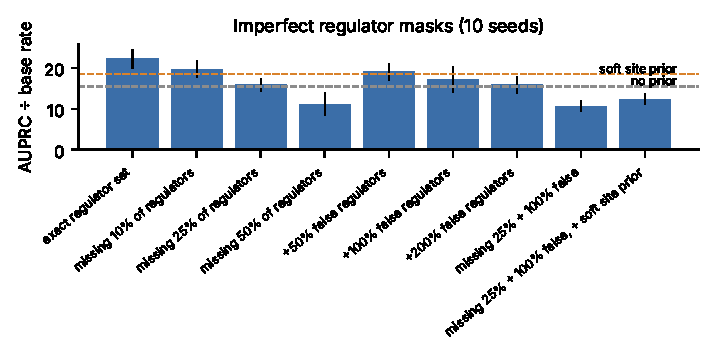
\includegraphics[width=0.6\textwidth]{figures/s_masks.pdf}
\caption{\textbf{Imperfect regulator masks.}}\label{fig:s_masks}\end{figure}

\subsection*{S8. Propagation depth: true vs estimated operator}
We evaluated every regulator (seeds 0--9), stratified by its true downstream depth, and scored both operators against the \emph{same} targets on the \emph{same} log-normalised scale (Table~\ref{tab:s_depth2}, Fig.~\ref{fig:s_depth}).
\begin{itemize}
\item \textbf{Targets:} (i) the noise-free steady-state knockdown effect, mapped to the log scale with the first-order transform of the simulator's normalisation; (ii) the measured mean effect in the simulated data.
\item \textbf{True operator:} the linearised production Jacobian at the wild-type steady state, with its predictions mapped to log scale by the same transform.
\item \textbf{Estimated operator:} BOND-V, 5-fold over knockdowns.
\end{itemize}
Remaining mismatches between the two operators include linearisation error, and cell-to-cell heterogeneity (input levels, cell size) that the true operator, computed at mean inputs, ignores. The noise-free and measured targets correlate 0.79 on average.

For regulators with downstream depth $\ge3$, the mean over $D\in\{2,3,4\}$ minus $D=1$ (bootstrap 95\% CI over 82 regulators) was:
\begin{itemize}
\item true operator: $+0.19$ [0.16, 0.23] against the noise-free target and $+0.07$ [0.05, 0.09] against the measured target;
\item estimated operator, stabilised (rescaled to spectral radius 0.8): $+0.04$ [0.01, 0.07] against the noise-free target and $-0.02$ [$-0.05$, $-0.00$] against the measured target;
\item estimated operator, unstabilised: strongly negative ($-0.35$ and $-0.51$).
\end{itemize}
\textbf{Conclusion:} deeper propagation helps with the true operator in this simulator, against both noise-free and measured targets. The estimated pipeline does not reproduce that benefit: there is no consistent improvement beyond one step after stabilisation, and collapse without it.
At $D=1$ on the measured target, the estimated operator matched or exceeded the true operator (0.70 vs 0.64 for deep regulators), consistent with the heterogeneity mismatch above. Table~\ref{tab:s_depth} reports the earlier comparison, in which the true operator was scored on noise-free raw-scale effects.
In Table~\ref{tab:s_f5depth}, the $(I-J)^{-1}$ column is an algebraic inverse. It equals the infinite propagation sum only when $\rho(J)<1$, which holds only for the stabilised rows.

\begin{table}[h]\centering\small
\caption{\textbf{Propagation depth, both operators on the same targets and scale} (correlation with the knockdown effect; mean over regulators; seeds 0--9).}\label{tab:s_depth2}
\resizebox{\textwidth}{!}{\begin{tabular}{lllcccccc}
\toprule
Operator & target & regulators (n) & $D{=}1$ & 2 & 3 & 4 & 6 & 8 \\
\midrule
true operator & noise-free & depth 1 (95) & 0.91 & 0.91 & 0.91 & 0.91 & 0.91 & 0.91 \\
true operator & noise-free & depth 2 (43) & 0.78 & 0.88 & 0.88 & 0.88 & 0.88 & 0.88 \\
true operator & noise-free & depth $\ge3$ (82) & 0.57 & 0.73 & 0.77 & 0.78 & 0.78 & 0.78 \\
true operator & measured & depth 1 (95) & 0.71 & 0.71 & 0.71 & 0.71 & 0.71 & 0.71 \\
true operator & measured & depth 2 (43) & 0.71 & 0.75 & 0.75 & 0.75 & 0.75 & 0.75 \\
true operator & measured & depth $\ge3$ (82) & 0.64 & 0.70 & 0.71 & 0.71 & 0.71 & 0.71 \\
estimated & noise-free & depth 1 (95) & 0.39 & 0.18 & 0.06 & 0.04 & 0.01 & -0.00 \\
estimated & noise-free & depth 2 (43) & 0.55 & 0.38 & 0.08 & -0.00 & 0.05 & -0.03 \\
estimated & noise-free & depth $\ge3$ (82) & 0.57 & 0.54 & 0.20 & -0.06 & 0.06 & -0.04 \\
estimated & measured & depth 1 (95) & 0.36 & 0.16 & 0.05 & 0.02 & 0.00 & -0.01 \\
estimated & measured & depth 2 (43) & 0.58 & 0.37 & 0.07 & -0.01 & 0.06 & -0.06 \\
estimated & measured & depth $\ge3$ (82) & 0.70 & 0.54 & 0.12 & -0.10 & 0.10 & -0.05 \\
estimated, stabilised & noise-free & depth 1 (95) & 0.39 & 0.33 & 0.31 & 0.33 & 0.33 & 0.33 \\
estimated, stabilised & noise-free & depth 2 (43) & 0.55 & 0.53 & 0.50 & 0.50 & 0.51 & 0.51 \\
estimated, stabilised & noise-free & depth $\ge3$ (82) & 0.57 & 0.63 & 0.62 & 0.61 & 0.61 & 0.61 \\
estimated, stabilised & measured & depth 1 (95) & 0.36 & 0.30 & 0.29 & 0.30 & 0.30 & 0.30 \\
estimated, stabilised & measured & depth 2 (43) & 0.58 & 0.55 & 0.51 & 0.51 & 0.52 & 0.52 \\
estimated, stabilised & measured & depth $\ge3$ (82) & 0.70 & 0.71 & 0.67 & 0.66 & 0.68 & 0.68 \\
\bottomrule
\end{tabular}
% corr(noise-free, measured targets) mean 0.79; 10 seeds}\end{table}
\begin{table}[h]\centering\small
\caption{\textbf{Propagation depth, earlier comparison on different targets} (true operator: noise-free raw-scale effects; estimated: measured log-scale effects). Superseded by Table~\ref{tab:s_depth2}.}\label{tab:s_depth}
\begin{tabular}{llcccccc}
\toprule
Operator & held-out regulators (n) & $D{=}1$ & 2 & 3 & 4 & 6 & 8 \\
\midrule
true operator & downstream depth 1 (95) & 0.90 & 0.90 & 0.90 & 0.90 & 0.90 & 0.90 \\
true operator & depth 2 (43) & 0.76 & 0.85 & 0.85 & 0.85 & 0.85 & 0.85 \\
true operator & depth $\ge3$ (82) & 0.61 & 0.74 & 0.78 & 0.78 & 0.78 & 0.78 \\
estimated & downstream depth 1 (95) & 0.36 & 0.16 & 0.05 & 0.02 & 0.00 & -0.01 \\
estimated & depth 2 (43) & 0.58 & 0.37 & 0.07 & -0.01 & 0.06 & -0.06 \\
estimated & depth $\ge3$ (82) & 0.70 & 0.54 & 0.12 & -0.10 & 0.10 & -0.05 \\
estimated, stabilised & downstream depth 1 (95) & 0.36 & 0.30 & 0.29 & 0.30 & 0.30 & 0.30 \\
estimated, stabilised & depth 2 (43) & 0.58 & 0.55 & 0.51 & 0.51 & 0.52 & 0.52 \\
estimated, stabilised & depth $\ge3$ (82) & 0.70 & 0.71 & 0.67 & 0.66 & 0.68 & 0.68 \\
\bottomrule
\end{tabular}
% 10 seeds; true operator spectral radius mean 0.00\end{table}
\begin{table}[h]\centering\small
\caption{\textbf{Truncated propagation on the four held-out knockdowns of the original design} (seeds 0--9). \textsuperscript{a}Algebraic inverse; equals the infinite sum only if $\rho(J)<1$.}\label{tab:s_f5depth}
\resizebox{\textwidth}{!}{\begin{tabular}{p{4.2cm}ccccccccc}
\toprule
Model & $D{=}1$ & 2 & 3 & 4 & 6 & 8 & 12 & $(I-J)^{-1}$\textsuperscript{a} & $\rho(J)$ \\
\midrule
no prior & 0.50 & 0.27 & 0.09 & 0.00 & 0.03 & -0.01 & -0.01 & 0.15 & 3.03 \\
hard identity mask + soft site prior & 0.41 & 0.21 & 0.14 & 0.08 & 0.06 & 0.00 & -0.01 & 0.18 & 2.53 \\
no prior, stabilised ($\rho$=0.8) & 0.50 & 0.45 & 0.43 & 0.45 & 0.44 & 0.44 & 0.44 & 0.44 & 0.80 \\
hard identity mask + soft site prior, stabilised ($\rho$=0.8) & 0.41 & 0.35 & 0.35 & 0.35 & 0.35 & 0.35 & 0.35 & 0.35 & 0.80 \\
\bottomrule
\end{tabular}}\end{table}
\begin{figure}[h]\centering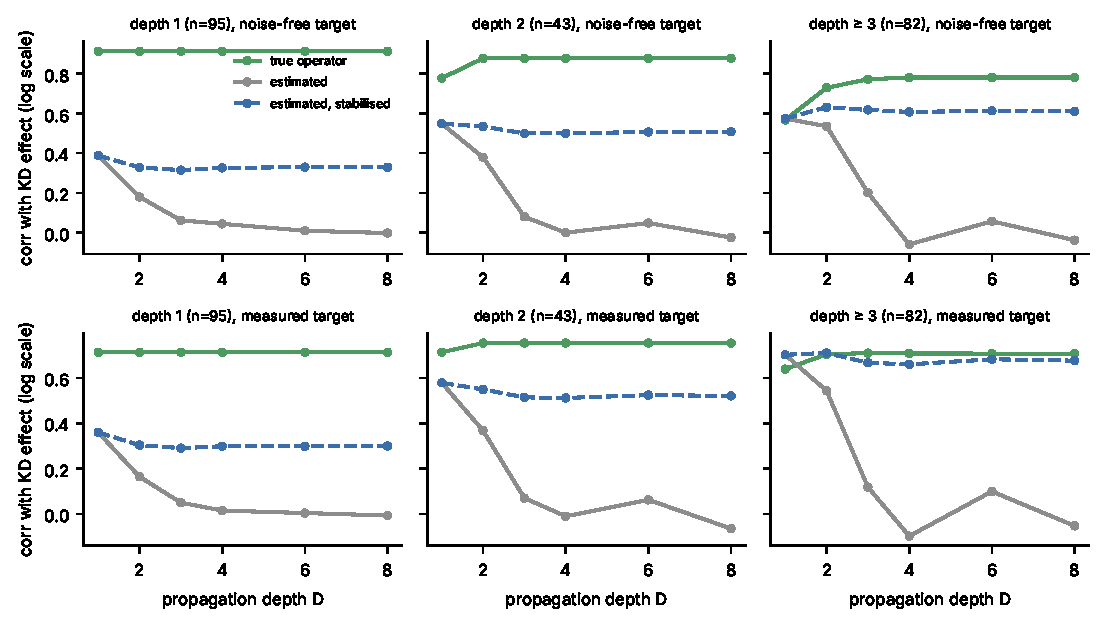
\includegraphics[width=\textwidth]{figures/s_depth_control.pdf}
\caption{\textbf{Propagation depth with the true vs estimated operator,} both scored against the same noise-free (top) and measured (bottom) log-scale targets, stratified by each regulator's true downstream depth.}\label{fig:s_depth}\end{figure}

\subsection*{S9. Context: earlier sign-flip summary and Shifrut 2018}
Table~\ref{tab:s_f6} gives a sign-flip summary that conditions on targets strong in both contexts; Table~\ref{tab:context} gives the unconditional, noise-matched analysis.

\begin{table}[h]\centering\small
\caption{\textbf{Sign flips among strong shared targets} (conditional analysis). Gain slope: total-least-squares slope of context-2 on context-1 effects.}\label{tab:s_f6}
\resizebox{\textwidth}{!}{\begin{tabular}{lcccccc}
\toprule
Comparison & $n$ & sign flips / strong shared & Jaccard & corr top-50 & gain slope (median) & fold gain change \\
\midrule
\multicolumn{7}{l}{\emph{Norman 2019 (K562, CRISPRa; from earlier analysis)}} \\
A alone vs A in C's context & 260 & -- (1.5\%) & 0.185 & -- & -- & -- \\
A alone, split-half null & 251 & -- (0.0\%) & 0.430 & -- & -- & -- \\
Cell-cycle state bins & 152 & 5/10223 (0.05\%) & -- & 0.96 & -- & 1.26 \\
\midrule \multicolumn{7}{l}{\emph{Wessels 2023 (THP-1, Cas13 knockdown)}} \\
A alone vs A in C's context & 106 & 18/1657 (1.09\%) & 0.106 & 0.44 & 0.99 & 1.20 \\
A alone, split-half null & 106 & 1/1463 (0.07\%) & 0.110 & 0.85 & 1.00 & 1.12 \\
\midrule \multicolumn{7}{l}{\emph{Shifrut 2018 (primary T cells, CRISPR KO)}} \\
No stimulation vs stimulation & 18 & 0/6 (0.00\%) & 0.011 & 0.02 & -- & -- \\
split-half null (no stim.) & 18 & 0/6 (0.00\%) & 0.010 & -0.02 & -- & -- \\
split-half null (stim.) & 18 & 0/12 (0.00\%) & 0.020 & 0.12 & -- & -- \\
\bottomrule
\end{tabular}}\end{table}

\subsection*{S10. Additional checks for the main-text analyses}
\begin{table}[h]\centering\small
\caption{\textbf{Noise-constant estimators.} Pooled and median per-knockdown expected-noise shares under alternative estimators of the noise constant, and a bootstrap over the 585 non-targeting controls (median estimator). Per-gene medians of squared z-scores are biased low for chi-square-like distributions and are shown divided by the $\chi^2_1$ median (0.455).}\label{tab:s_noise}
\begin{tabular}{lcc}
\toprule
Noise-constant estimator & pooled noise share & median per-knockdown noise share \\
\midrule
median over controls (used) & 0.470 & 0.737 \\
mean over controls & 0.499 & 0.782 \\
20\% trimmed mean & 0.471 & 0.738 \\
gene-specific mean & 0.499 & 0.782 \\
gene-specific median / chi2 median (0.455) & 0.475 & 0.745 \\
Bootstrap over 585 controls (95\% interval, median estimator) & [0.467, 0.473] & [0.733, 0.742] \\
\bottomrule
\end{tabular}\end{table}
\begin{table}[h]\centering\small
\caption{\textbf{Matched shared axes across screens} ($|\cos|$ between individual axes fitted separately in each screen on the 1{,}457 knockdowns in both).}\label{tab:s_pcmatch}
\begin{tabular}{lccc}
\toprule
GW axis $\backslash$ essential axis & 1 & 2 & 3 \\
\midrule
1 & 0.95 & 0.17 & 0.08 \\
2 & 0.16 & 0.91 & 0.13 \\
3 & 0.05 & 0.12 & 0.02 \\
\bottomrule
\end{tabular}\end{table}
\begin{table}[h]\centering\small
\caption{\textbf{Positive-control robustness.} Mean difference between cascade and random-mediator correlations for semi-synthetic targets with exact cascade share $\alpha$ (realised share equals nominal in orthogonalised generators; in the non-orthogonal generator the realised share was 0.005, 0.053, 0.102, 0.250 and 0.499). $^\ast$: 95\% CI lower bound above the real-data upper bound (0.004).}\label{tab:s_pc2}
\resizebox{\textwidth}{!}{\begin{tabular}{p{6.2cm}cccccc}
\toprule
Generator & coverage & \multicolumn{5}{c}{cascade share $\alpha$ (exact energy fraction)} \\
 & & 0 & 0.05 & 0.1 & 0.25 & 0.5 \\
\midrule
base (orthogonal, strongest mediators, coordinates restored, equal reliability) & 1.0 & 0.000 & 0.047$^\ast$ & 0.066$^\ast$ & 0.106$^\ast$ & 0.153$^\ast$ \\
base (orthogonal, strongest mediators, coordinates restored, equal reliability) & 0.25 & -0.002 & 0.008$^\ast$ & 0.013$^\ast$ & 0.026$^\ast$ & 0.039$^\ast$ \\
mediators ranked at random (ranking errors) & 1.0 & -0.003 & 0.006 & 0.009$^\ast$ & 0.017$^\ast$ & 0.023$^\ast$ \\
mediators ranked at random (ranking errors) & 0.25 & -0.003 & -0.001 & -0.001 & 0.003 & 0.005 \\
mediator coordinates not restored & 1.0 & -0.004 & -0.002 & -0.002 & -0.000 & 0.001 \\
mediator coordinates not restored & 0.25 & 0.000 & -0.001 & -0.002 & -0.003 & 0.001 \\
heterogeneous mediator strengths (lognormal, sd 1) & 1.0 & -0.003 & 0.035$^\ast$ & 0.049$^\ast$ & 0.080$^\ast$ & 0.115$^\ast$ \\
heterogeneous mediator strengths (lognormal, sd 1) & 0.25 & -0.004 & 0.003 & 0.008$^\ast$ & 0.015$^\ast$ & 0.027$^\ast$ \\
screen-2 reliability halved & 1.0 & 0.000 & 0.033$^\ast$ & 0.046$^\ast$ & 0.074$^\ast$ & 0.107$^\ast$ \\
screen-2 reliability halved & 0.25 & -0.001 & 0.005 & 0.009$^\ast$ & 0.018$^\ast$ & 0.027$^\ast$ \\
screen-1 reliability halved & 1.0 & -0.003 & 0.032$^\ast$ & 0.047$^\ast$ & 0.074$^\ast$ & 0.109$^\ast$ \\
screen-1 reliability halved & 0.25 & -0.003 & 0.006 & 0.009$^\ast$ & 0.018$^\ast$ & 0.026$^\ast$ \\
non-orthogonal construction (original) & 1.0 & -0.002 & 0.044$^\ast$ & 0.064$^\ast$ & 0.104$^\ast$ & 0.152$^\ast$ \\
non-orthogonal construction (original) & 0.25 & -0.003 & 0.008$^\ast$ & 0.013$^\ast$ & 0.025$^\ast$ & 0.038$^\ast$ \\
all adverse: random ranking, no restore, heterogeneous, screen-2 halved & 1.0 & -0.001 & -0.003 & -0.003 & -0.001 & -0.000 \\
all adverse: random ranking, no restore, heterogeneous, screen-2 halved & 0.25 & -0.003 & -0.004 & -0.004 & -0.001 & -0.001 \\
\midrule
Real data (specific residual) & -- & \multicolumn{5}{c}{-0.004 [-0.012, 0.004]} \\
\bottomrule
\end{tabular}}\end{table}
\begin{table}[h]\centering\small
\caption{\textbf{Calibrated magnitude scores} on independent-screen targets ($R^2_0$ uncalibrated; after training-only scalar calibration with bootstrap 95\% CI; mean calibration factor $\bar\lambda$ over folds).}\label{tab:s_f2cal}
\resizebox{\textwidth}{!}{\begin{tabular}{l ccc ccc ccc}
\toprule
 & \multicolumn{3}{c}{Indep., raw} & \multicolumn{3}{c}{Indep., mean-centred} & \multicolumn{3}{c}{Indep., specific} \\
Predictor & $R^2_0$ & $R^2_0$ calibrated [95\% CI] & $\bar\lambda$ & $R^2_0$ & calibrated & $\bar\lambda$ & $R^2_0$ & calibrated & $\bar\lambda$ \\
\midrule
mean training profile & 0.007 & 0.033 [0.029, 0.036] & 0.53 & 0.000 & 0.000 [0.000, 0.000] & 0.00 & -0.000 & -0.000 [-0.000, 0.000] & 8.00 \\
kNN k=10 & -0.189 & 0.037 [0.032, 0.042] & 0.28 & -0.174 & 0.006 [0.004, 0.009] & 0.15 & -0.120 & 0.002 [0.001, 0.003] & 0.10 \\
kNN k=20 & -0.117 & 0.042 [0.036, 0.048] & 0.35 & -0.106 & 0.007 [0.003, 0.010] & 0.20 & -0.056 & 0.003 [0.002, 0.003] & 0.16 \\
kNN k=50 & -0.064 & 0.046 [0.040, 0.052] & 0.40 & -0.056 & 0.006 [0.002, 0.010] & 0.26 & -0.017 & 0.004 [0.003, 0.005] & 0.27 \\
kNN k=100 & -0.039 & 0.047 [0.041, 0.052] & 0.42 & -0.033 & 0.005 [0.002, 0.008] & 0.28 & -0.004 & 0.004 [0.003, 0.005] & 0.36 \\
factorised (generic mean + pathway kNN50 + specific kNN50) & -0.017 & 0.043 [0.037, 0.049] & 0.46 & -0.016 & 0.012 [0.009, 0.016] & 0.40 & -0.017 & 0.004 [0.003, 0.005] & 0.27 \\
\bottomrule
\end{tabular}}\end{table}
\begin{table}[h]\centering\small
\caption{\textbf{Paired predictor comparisons} (per-knockdown differences; bootstrap 95\% CI).}\label{tab:s_f2pairs}
\resizebox{\textwidth}{!}{\begin{tabular}{llcc}
\toprule
Paired comparison & target & $\Delta$ corr [95\% CI] & $\Delta R^2_0$ calibrated [95\% CI] \\
\midrule
kNN k=100 minus kNN k=10 & raw & 0.041 [0.034, 0.048] & 0.0097 [0.0064, 0.0127] \\
kNN k=100 minus kNN k=10 & mean-centred & 0.020 [0.009, 0.030] & -0.0011 [-0.0034, 0.0010] \\
kNN k=100 minus kNN k=10 & specific residual & 0.023 [0.016, 0.030] & 0.0024 [0.0016, 0.0031] \\
kNN k=50 minus kNN k=10 & raw & 0.040 [0.033, 0.046] & 0.0089 [0.0056, 0.0118] \\
kNN k=50 minus kNN k=10 & mean-centred & 0.022 [0.013, 0.031] & -0.0001 [-0.0024, 0.0020] \\
kNN k=50 minus kNN k=10 & specific residual & 0.016 [0.010, 0.022] & 0.0018 [0.0011, 0.0024] \\
kNN k=100 minus kNN k=50 & raw & 0.002 [-0.001, 0.004] & 0.0008 [-0.0005, 0.0022] \\
kNN k=100 minus kNN k=50 & mean-centred & -0.002 [-0.007, 0.003] & -0.0010 [-0.0019, 0.0000] \\
kNN k=100 minus kNN k=50 & specific residual & 0.007 [0.002, 0.011] & 0.0006 [0.0002, 0.0010] \\
factorised (generic mean + pathway kNN50 + specific kNN50) minus kNN k=50 & raw & -0.007 [-0.009, -0.005] & -0.0031 [-0.0048, -0.0012] \\
factorised (generic mean + pathway kNN50 + specific kNN50) minus kNN k=50 & mean-centred & 0.005 [-0.002, 0.012] & 0.0064 [0.0046, 0.0083] \\
factorised (generic mean + pathway kNN50 + specific kNN50) minus kNN k=50 & specific residual & 0.000 [-0.000, 0.000] & -0.0000 [-0.0000, 0.0000] \\
\bottomrule
\end{tabular}}\end{table}

\subsection*{S11. Reproducibility}
Environments: main-text and Supplement S5--S10 analyses were run with Python 3.13 and the versions in \texttt{requirements.txt}; Supplement S1--S4 (including the PyTorch latent-ODE runs) were run mainly on a second machine with Python 3.10.12 and the versions in \texttt{requirements-s1-s4.txt} (torch 2.14.1+cpu); some 80-gene coverage runs used the main environment. \texttt{run\_all.sh} lists the commands used, in order, starting from the raw files listed in \texttt{data/README.md}. End-to-end regeneration from a clean environment was verified only for the analyses stated in the main-text Methods; the other commands are supplied but not re-verified. Random seeds are fixed in each script (\texttt{numpy.random.default\_rng} with the seeds stated above). Approximate run times on a 2-core machine: decomposition and benchmark $<$10 min; cascade test with positive control about 10 min; 80-gene simulations 1--3 h.

